\documentclass[12pt]{article}
\usepackage[utf8]{inputenc} % default from sharelatex
\usepackage[a4paper, left=20mm, right=20mm, top=20mm, bottom=20mm]{geometry} % dont break my public key
\usepackage{indentfirst} % to indent fist paragraph
\usepackage[brazilian]{babel} % BR
\usepackage{hyperref} % to links
\usepackage{listings} % to code block
\usepackage{graphicx} % to have pictures

\graphicspath{{images/}}
\lstset{breaklines=true, basicstyle={\small\ttfamily},}

\title{Trabalho individual sobre PGP}
\author{Lucas João Martins}
\date{}

\begin{document}

\maketitle

\section*{}
\subsection*{1) Criar certificado pgp}
Chave pública publicada em \url{https://keyserver.pgp.com} com as seguintes características:

\begin{lstlisting}
pub   2048R/85325AA4 2017-08-16
Key fingerprint = 25EA 0F7C CF7A 1C7D D50D  C7D8 13A0 25BF 8532 5AA4
uid                  Lucas Joao Martins <lucasjoao.lj@gmail.com>
sub   2048R/BE9BF8A3 2017-08-16
\end{lstlisting}

Onde a chave pública é:

\begin{lstlisting}
-----BEGIN PGP PUBLIC KEY BLOCK-----
Version: GnuPG v1

mQENBFmUjDgBCADIOK5PuUrM+9WpsXG1OFzZ1AqGtdTmG8+2IQ8pJcOSLEX/Ve9E
R/5lrlgky6R5RquED+5QzLXmQI9syJOCwnGVh9f8eDE3YHUeJcnlpm49dpg8QhrI
2y5AD23Tq7LF9W9jP587GoojjPqGjTdnh+p3OApsHNigdvHbgeAI+5mPGlISWpub
wgf3Cyx4JCVPb5VQyO4SJx3f7mQ0qQy/va/rYatSnt7nEK4Fgae2E7Tn3Yu1wLXt
dzNcgvDQvaXxPWcDd1pnxDwYeoFBbxwp7Aj9Wxv/qmPJF57MoE/fYB6IDEuPd1R1
E9aLynv2xE3Mydgo+sbkz2N0Kr9+/KZWSgrDABEBAAG0LEx1Y2FzIEpvw6NvIE1h
cnRpbnMgPGx1Y2Fzam9hby5sakBnbWFpbC5jb20+iQE4BBMBAgAiBQJZlIw4AhsD
BgsJCAcDAgYVCAIJCgsEFgIDAQIeAQIXgAAKCRAToCW/hTJapN4GB/9gygLSm9+G
CUB3VBMrR2Soq/oo8Z0plVV5CyBZTFam8etBRZQoYVFxQabtmdNF0OILJjpQFmO2
YsxKjm9TglM4Rq9GS86/DfPT3KR6zy8i4e+vzfa6sshPH8WpTCRjhvjfq8XtLA4Z
MoZL2LLkn1bB7X2xsemOEoBNm8oza4f/xbMRWqmGPnTUBc/QiFOaCdar8Tqg0DyK
FBsieotHVNczioGlOkPnACUyfm/CcArJYHC7jyUVIg02Fh9bVb+iZ0BNGPNev4AD
DoEceOzv29CpSmbB48UXEcF+qUrT+Wu53BaqFB3kUj0rA3i9PRMql4MV+7+RpRf1
3nvSiPasZF0AuQENBFmUjDgBCADgaJ8b889Uj5s6Hhr7OLbTQ+Be4dtEd9l5v9y3
pN1PjEtw1WniA4TcQ1vWukflUoYysyU7pKKKmvOPqCtZrq91YEmylv5w14p6Mg6P
SbZEskQ1zduzbFXqCpvmoudgRDONCFHyYcemLpQNLxIAHSsxRP251exU9IFQyH4h
kBAmregLrIembWwFwG9l2RUBjRyY3maMEwVNKpg/B5kTTB6ORoFZLmmdWjWAXF5c
850RTW0zTWIlgAOlTx6huRdR0SWkExu4H6Cp4Gbbl6zBN3bcKu3RWburoiY3ui/F
uXy2WXWxCQBok95JT7rVfJTtXGGGi2zSLR8lxWL0YfmOqAQnABEBAAGJAR8EGAEC
AAkFAlmUjDgCGwwACgkQE6Alv4UyWqRK3wgAmX4TGrYHxr76jTl9cJf+Jdfjt+/n
LPIm2ZY1IRCZxAGo3rLNMXGKFaU53zIgXliQzQA+A7zRxKtjgldyF33BXTyOHexE
iq0XwUzRuYiWQzQ3RbRSDr5TlTF35VO1vNI30AKWvc0llyr9OYR0AWMPVaQyApHJ
lvxwJBugoENnqcIGVFAowI3mQCnxfbtOrqFVgc99qgvIuyvG3DZ02Ldx4dvVRZ+C
vqh+OZqsUCgLtKdDUBvQ8OqiL9oBiuqBcxsoQuWwt1O4QJgpAn5uklSAX/gu4SxS
y+VdBrgFI/os8dS8M3kI6xcnhVwfnKVRT1MfNmQ1a4ElpeRV7hPNv/BSmw==
=pHJb
-----END PGP PUBLIC KEY BLOCK-----
\end{lstlisting}

\subsection*{2) Crie um novo certificado PGP para este trabalho individual (Não use o teu certificado pois ele terá que ser revogado). Coloque esse certificado de testes no servidor PGP. Depois verifique seu status. Então, crie um certificado de revogação e revogue o certificado de testes.}
Nova chave pública também publicada em \url{https://keyserver.pgp.com} com as seguintes características:

\begin{lstlisting}
  pub   2048R/1EA6B159 2017-08-16 [expires: 2018-08-16]
  Key fingerprint = 56DA 97B8 B02B 7C23 7C86  82DD 41D6 74B6 1EA6 B159
  uid                  Lucas Joao Martins (trabalho ine5429) <lucas.joao@bridge.ufsc.br>
  sub   2048R/6992884F 2017-08-16 [expires: 2018-08-16]
\end{lstlisting}

Para confirmar o status:

\begin{figure}[h] % https://tex.stackexchange.com/questions/8652/what-does-t-and-ht-mean
  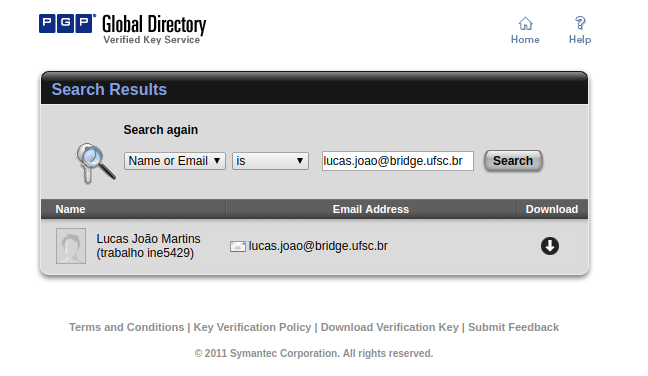
\includegraphics[width=\linewidth]{status01}
  \caption{Confirmação do status}
\end{figure}

Comprovação da revogação da chave pública criada:

\begin{lstlisting}
-----BEGIN PGP PUBLIC KEY BLOCK-----
Version: GnuPG v1
Comment: A revocation certificate should follow

iQEfBCABAgAJBQJZlJyJAh0DAAoJEEHWdLYeprFZP1wIAJ5DCG5YIJkSIS0FkUfo
93B/LOAVuIwQm/Tlmq60EoG6F1SCfGG8iORZlS5lLSr6JrV6wGGCuPFnrF63xegy
VRaZu/ANqzHjniHP92D3NlowwBvCz4yu+Pj448aGyS5FTfllQg+c3QnZoO/wMTaL
TsAH28OvtHsjjvOaEe+26/INUDEd8O8jGkDpGHlWzK3V8LJSDJAKUEBU4LnB58SJ
JtSlscm8r/Q/Wom959CbDSfsFYyuNapXMeyBbq7i1O4ZuNVVzN/c5FHa7vP7OsmH
mF7qYiCbO9EKbAZ4uGNhQ2uTun9Aq19ZheWgiG3/zGER7stDu3Z2rzRk7Aw2Vhp/
C3Q=
=npef
-----END PGP PUBLIC KEY BLOCK----
\end{lstlisting}

Por outro lado, no \url{https://keyserver.pgp.com} não é possível revogar uma chave. Segundo eles em \url{http://keyserver1.pgp.com/vkd/VKDHelpPGPCom.html}: ``\textit{Can I post a revoked key to the PGP Global Directory?} No. The PGP Global Directory includes many features to prevent it from being filled with unusable keys. One of these features is that the directory does not support revoked keys. Instead of revoking your key, simply remove it from the directory.''

\subsection*{3) Pratique a revogação de certificados PGP. Assine um certificado qualquer PGP ( de outra pessoa ). E envie esse certificado para o servidor PGP. Depois verifique o status do certificado. E então, revogue a assinatura que você fez. Confira o resultado no servidor PGP. Faça um relatório do que você fez, incluindo o KeyID do certificado cuja assinatura você revogou.}
Chave pública utilizada de outra pessoa:

\begin{lstlisting}
pub   2048R/E14C3A8A 2017-06-30
uid                  John <asdfedc@mail.com>
sub   2048R/0F6A27DC 2017-06-30
\end{lstlisting}

Saída do comando \lstinline{gpg --list-sigs asdfedc@mail.com} que mostra a assinatura da chave pública:

\begin{lstlisting}
pub   2048R/E14C3A8A 2017-06-30
uid                  John <asdfedc@mail.com>
sig      N   E14C3A8A 2017-06-30  John <asdfedc@mail.com>
sig          CA57AD7C 2017-08-09  [User ID not found]
sig 1        85325AA4 2017-08-16  Lucas Joao Martins <lucasjoao.lj@gmail.com>
sub   2048R/0F6A27DC 2017-06-30
sig          E14C3A8A 2017-06-30  John <asdfedc@mail.com>
\end{lstlisting}

Saída do comando \lstinline{gpg --edit-key asdfedc@mail.com} que mostra o processo para revogar a assinatura realizada anteriormente:

\begin{lstlisting}
gpg (GnuPG) 1.4.20; Copyright (C) 2015 Free Software Foundation, Inc.
This is free software: you are free to change and redistribute it.
There is NO WARRANTY, to the extent permitted by law.


pub  2048R/E14C3A8A  created: 2017-06-30  expires: never       usage: SC
                     trust: unknown       validity: unknown
sub  2048R/0F6A27DC  created: 2017-06-30  expires: never       usage: E
[ unknown] (1). John <asdfedc@mail.com>

gpg> revsig
You have signed these user IDs on key E14C3A8A:
     John <asdfedc@mail.com>
   signed by your key 85325AA4 on 2017-08-16

user ID: "John <asdfedc@mail.com>"
signed by your key 85325AA4 on 2017-08-16
Create a revocation certificate for this signature? (y/N) y
You are about to revoke these signatures:
     John <asdfedc@mail.com>
   signed by your key 85325AA4 on 2017-08-16
Really create the revocation certificates? (y/N) y
Please select the reason for the revocation:
  0 = No reason specified
  4 = User ID is no longer valid
  Q = Cancel
Your decision? 0
Enter an optional description; end it with an empty line:
>
Reason for revocation: No reason specified
(No description given)
Is this okay? (y/N) y

You need a passphrase to unlock the secret key for
user: "Lucas Joao Martins <lucasjoao.lj@gmail.com>"
2048-bit RSA key, ID 85325AA4, created 2017-08-16

pub  2048R/E14C3A8A  created: 2017-06-30  expires: never       usage: SC
trust: unknown       validity: unknown
sub  2048R/0F6A27DC  created: 2017-06-30  expires: never       usage: E
[ unknown] (1). John <asdfedc@mail.com>

gpg> exit
\end{lstlisting}

Saída do comando \lstinline{gpg --list-sigs asdfedc@mail.com --verbose} que mostra a revogação da assinatura na chave pública:

\begin{lstlisting}
pub   2048R/E14C3A8A 2017-06-30
uid                  John <asdfedc@mail.com>
rev          85325AA4 2017-08-16  Lucas Joao Martins <lucasjoao.lj@gmail.com>
sig      N   E14C3A8A 2017-06-30  John <asdfedc@mail.com>
sig          CA57AD7C 2017-08-09  [User ID not found]
sig 1        85325AA4 2017-08-16  Lucas Joao Martins <lucasjoao.lj@gmail.com>
sub   2048R/0F6A27DC 2017-06-30
sig          E14C3A8A 2017-06-30  John <asdfedc@mail.com>
\end{lstlisting}

\subsection*{4) O que é o anel de chaves privadas? Como este está estruturado? Na sua aplicação GPG onde este anel de chaves é armazenado? Quem pode ser acesso a esse porta chaves?}
O anel de chaves privadas, também conhecido como private key ring, é um arquivo que possui as chaves privadas associadas à aplicação GPG. Trata-se de um arquivo binário no formato .gpg que fica localizado no \lstinline{/home}, mais precisamente em \lstinline{~/.gnupg/secring.gpg}. A string de permissão desse arquivo é \lstinline{-rw-------}, ou seja, somente o proprietário pode acessar ele.

\subsection*{5) Qual a diferença entre assinar uma chave local e assinar no servidor?}
Somente assinar a chave localmente faz com que as outras pessoas não saibam automaticamente que uma chave pública foi assinada, pois sem um servidor, quando Bob assina a chave de Alice ele precisa enviar a chave pública dela que foi assinada para Alice, para que assim ela possa atualizar sua chave pública e distribuir para todos os seus correspondentes. Por outro lado, ao assinar a chave no servidor, pode-se dizer, de maneira resumida, que esse processo é automatizado sem a necessidade que Alice participe da distribuição da sua chave pública.

\subsection*{6) O que é e como é organizado o banco de dados de confiabilidade?}
Um banco de dados de confiabilidade é um arquivo que possui as chaves públicas de outras pessoas nas quais o usuário confia. Vale citar que quando uma chave pública de outra pessoa é assinada o assinante deve escolher, dentro de quatro opções, um nível de confiança dele naquela chave. O nível de confiança escolhido pode implicar na adição ou na exclusão de chaves públicas, no banco de dados de confiabilidade, assinadas pela chave pública que está sendo assinada pelo assinante. Essa ideia está associada ao conceito de web of trust.

\subsection*{7) O que são e para que servem as sub-chaves?}
Sub-chaves são como chaves normais, exceto pelo fato que elas são sempre associadas a um par de chaves normais, chamado de par mestre de chaves. Subchaves podem ser utilizadas para assinaturas e ciframento. A grande vantagem de utilizar subchave é que elas podem ser revogadas sem afetar seu par mestre de chaves, além da possibilidade de serem armazenadas em locais diferentes.

\subsection*{8) Coloque sua foto ( ou uma figura qualquer ) que represente você em seu certificado GPG.}
\begin{figure}[!h] % https://tex.stackexchange.com/questions/8652/what-does-t-and-ht-mean
  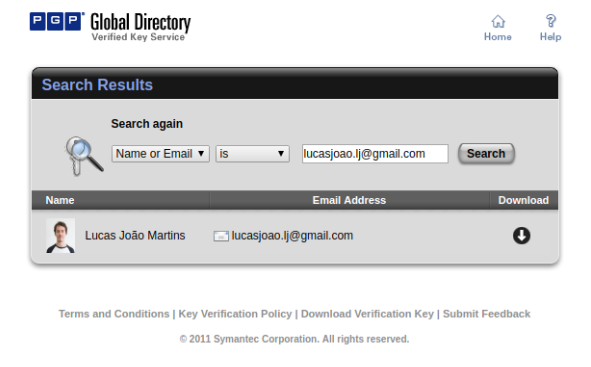
\includegraphics[width=\linewidth, height=9cm]{status02}
  \caption{Foto pessoal na chave pública}
\end{figure}

\subsection*{9) O que é preciso para criar e manter um servidor de chaves GPG, sincronizado com os demais servidores existentes?}
Para manter um próprio servidor de chaves GPG sincronizado com outros servidores é necessário ter acesso aos dumps de chaves desses outros servidores, pois dessa forma seria possível adicionar a base de chaves do servidor próprio as chaves presentes nesse backup. Entretanto, na prática, segundo alguns ``guias de como construir o seu próprio servidor de chaves'' apenas poucos servidores disponibilizam esses backups gratuitamente para download, e, quando fazem costumam possuir um processo semanal de atualização do dump.

\subsection*{10) Dê um exemplo de como tornar sigiloso um arquivo usando o GPG.}
Através do comando \lstinline{gpg -e -r id file}. Onde \lstinline{-e} significa para cifrar o \lstinline{file} e o \lstinline{-r} significa que irá cifrar com a chave do \lstinline{id}. Isso irá gerar um arquivo cifrado com a extensão \lstinline{.gpg}.

\subsection*{11) Dê um exemplo de como assinar um arquivo ( assinatura anexada e outro com assinatura separada ), usando o GPG}
Para realizar uma assinatura anexada, precisa-se utilizar o comando \break \lstinline{gpg --output arquivo_de_saida --clearsign arquivo_de_entrada}. Com isso, um \break \lstinline{arquivo_de_saida} ASCII vai ser gerado com o arquivo em si e com a assinatura digital. Já para realizar uma assinatura separada, deve-se utilizar o \break \lstinline{gpg --armor --detach-sig arquivo_de_entrada}. Desse modo, um \lstinline{arquivo_de_entrada.asc} vai ser criado com a assinatura.
\end{document}
